\section{Моделирование передачи сигналов, заданных отсчетами во временной области}
\label{sec:model}
	Сигнал на выходе канала с АБГШ задается выражением
	\begin{equation}
	\label{Glebov.f1}
		r(t)=s_i(t)+n(t),
	\end{equation}
	где $0<t<T_s$ - длительность сигнала, $i=0,1,...,q-1$ - количество сигналов.

	Отношение сигнал/шум определяется как
	\begin{equation}
	\label{Glebov.f2}
		\frac{E}{N_0}=\frac{1}{N_0}\frac{1}{q}\sum_{i=0}^{\infty}E_i,
	\end{equation}
	где $E_i$ - энергия $i$-го сигнала.
	
	Для моделирования передачи по каналу с шумом, заданному выражением
	\ref{Glebov.f1}, представим принятый сигнал как последовательность отсчетов, всзятых с интервалом $\Delta_t$, то есть
	\begin{equation}
	\label{Glebov.f3}
		r^{(l)}=s_i^{(l)}+n^{(l)},
	\end{equation}
	где $r^{(l)}=r(\Delta_t)$-отсчет сигнала на выходе канала, $s_i^{(l)}=s_i(\Delta_t)$-отсчет переданного сигнала,
	 $l=1,2,...,N_s$, $N_s$-количество отсчетов, $\Delta_t=T_s/N_s$. В канале с АБГШ $n^{(l)}$ это гауссовская 
	 случайная величина с параметрами $\overline{n^{(l)}}=0$ и $\overline{(n^{(l)})^2}=\sigma^2$. 
	 Для последующего моделирования случайной величины $n^{(l)}$ необходимо определить значение дисперсии
	 отсчета $\sigma^2$ и связать его с соотношением сигнал/шум.
	
	Энергия сигнала представленного дискретными отсчетами равна
	\begin{equation}
	\label{Glebov.f4}
		E_i=\sum_{l=1}^{N_s}(s_i^{(l)})^2\Delta_t.
	\end{equation}
	
	Случайная величина $n_j$, где $j=1,2,...,D$, $D$-размерность сигнального пространства, 
	определятеся как $n_j=\int_{0}^{T_s}n(t)\varphi_j(t)dt$, где $\varphi_j(t)$-базисная ортонормированная функция. 
	Параметры величины $n_j$ следующие $\overline{n_j}=0$ и 
	\begin{equation}
	\label{Glebov.f5}
		\overline{n_j^2}=N_0/2.
	\end{equation}
	Для базисной функции, заданной отсчетами, получим
	\begin{equation}
	\label{Glebov.f6}
	\begin{split}
		 n_j=\int_{0}^{T_s}n(t)\varphi_j(t)dt\approx\sum_{l=1}^{N_s}\int_{(l-1)\Delta_t}^{l\Delta_t}n(t)\varphi_j(l\Delta_t)dt=\sum_{l=1}^{N_s}\int_{(l-1)\Delta_t}^{l\Delta_t}n(t)\varphi_j^{(l)}dt= \\		 
		  =\sum_{l=1}^{N_s}\varphi_j^{(k)}\int_{(l-1)\Delta_t}^{l\Delta_t}n(t)dt=\sum_{l=1}^{N_s}\varphi_j^{(l)}\xi^{(l)},
	\end{split}	
	\end{equation}
	где $\xi^{(l)}=\int_{(l-1)\Delta_t}^{l\Delta_t}n(t)dt$-гауссовская случайная величина с нулевым средним и дисперсией
	\begin{equation}
	\label{Glebov.f7}
		\varphi_\xi^2=(N_0/2)\Delta_t
	\end{equation}
	
	При большом числе отсчетов $N_s$ длительность интервала дискритизации $\Delta_t$ будет уменшьаться, тогда выполняется равенство
	\begin{equation}
	\label{Glebov.f8}
		n_j=\int_{0}^{T_s}n(t)\varphi_j(t)dt\approx\sum_{l=1}^{N_s}n^{(l)}\varphi_j(l\Delta_t)\Delta_t,
	\end{equation}
	Из \ref{Glebov.f5}, \ref{Glebov.f6}, \ref{Glebov.f7} и \ref{Glebov.f8} следует,
	что $n^{(l)}\Delta_t=\xi^{(l)}$. Тогда, $\sigma_j=\overline{(n^{(l)})^2}=\sigma_j^2/\Delta_t^2=(N_0/2)/\Delta_t$, 
	далее $N_0/2=\sigma^2\Delta_t$. Тогда из формулы \ref{Glebov.f2} получаем, что
	\begin{equation}
	\frac{E}{N_0}=\frac{1}{2\sigma^2\Delta_t}\frac{1}{q}\sum_{i=0}^{q-1}E_i
	\end{equation}
	Отсюда получаем значение дисперсии шума
	\begin{equation}
		\sigma^2=\frac{1}{2(E/N_0)}\frac{1}{q}\sum_{i=0}^{q-1}\sum_{l=1}^{N_s}(s_i^{(l)})^2
	\end{equation}
	
	Для моделирования передачи по каналу с АБГШ нужно использовать гуассовские псевдослучайные величины с дисперсией 
	$\sigma^2$.
	
	\section{Вероятность ошибки в двоичном канале с АБГШ моделирующая программа}
	Схема передачи в двоичном канале выглядит следующим образом
	\begin{figure}[h]
		\centering
		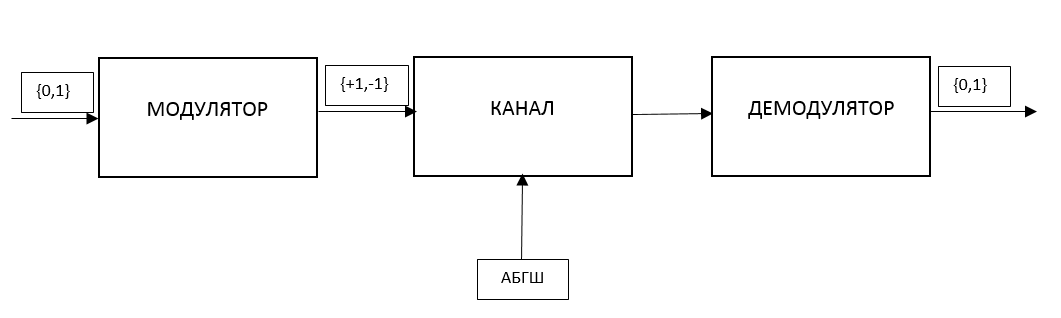
\includegraphics[scale=0.5]{img/Glebov_1.png}
		\caption{Схема передачи в двоичном канале с АБГШ}
		\label{Glebov.image1}
	\end{figure}
	
	Сообщения для предачи $\{0,1\}$ поступают на вход модулятора, где они преобразуются в сигналы вида 
	$\{-1,+1\}$, $0$ модулируется сигналом $-1$, $1$ модулируется сигналом $+1$, , 
	далее сигнал поступает в канал, где к нему добавляется аддитивный белый гауссовский шум. 
	Полученный сигнал поступает на вход демодулятора(приемника), который решает какое передавалось сообщение.
	
	Приемник работает следующим образом. Из принятого сигнала выбирает $K$ отсчтеов, далее вычисляется сумма
	\begin{equation}
		sum=\sum_{i=1}^{K}s_i,
	\end{equation}
	где $s_i$ - $i$-ый отсчет сигнлала.
	
	Если $sum>0$ приемник решает, что передавался сигнал $+1$, если $sum<0$, значит $-1$. 
	Сигналу $+1$ ставится в соостветсвие сообщение $1$, а сигналу $-1$, стваится $0$.
	
	Для оценки вероятности ошибки для различного количества отсчетов $K$ была написана моделирующая программаю.
	
	Результат программы:
	\begin{figure}[h]
		\centering
		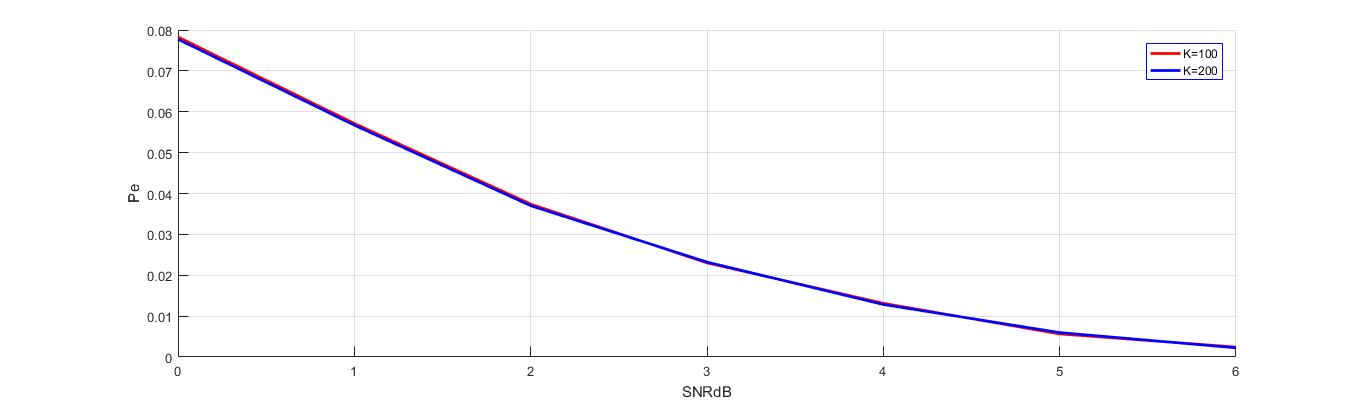
\includegraphics[scale=0.4]{img/Glebov_g.png}
		\caption{Вероятность ошибки}
		\label{Glebov.image2}
	\end{figure}
	
	Из графика видно, что вероятность ошибки не зависит от числа взятых отсчетов.
	
	\section{Схама формирования и приема сигналов в комплексной форме. (Почему не нужно использовать интегратор)}
	Рассмотрим схему формирования комплексного сигнала на примере передачи сообщения.
	
	\begin{itemize}
		\item сообщение абонента $i$ отображается на точку в сигнальном созвездии КАМ(ФМ), пара коэфициентов $(s_1,s_2)$ определяют эту точку;
		\item из полученных коэфициентов формируется вектор $X=s_1+js_2$;
		\item по вектору $X$ вычисляется комплексный вектор $x$ (быстрое ДПФ);
		\item по $Re\ x$ и $Im\ x$ восстанавливаются непрерывные сигналы $Re\ x(t)$ и $Im\ x(t)$ (цифро-аналоговое преобразование и интерполяция);
		\item формируется сигнал $Re\ x(t)\varphi_1-Im\ x(t)\varphi_2$, где $\varphi_1=\sqrt{2/T}\cos2\pi f_0t$ и  $\varphi_2=-\sqrt{2/T}\sin2\pi f_0t$
	\end{itemize}
	
	\begin{figure}[h]
		\centering
		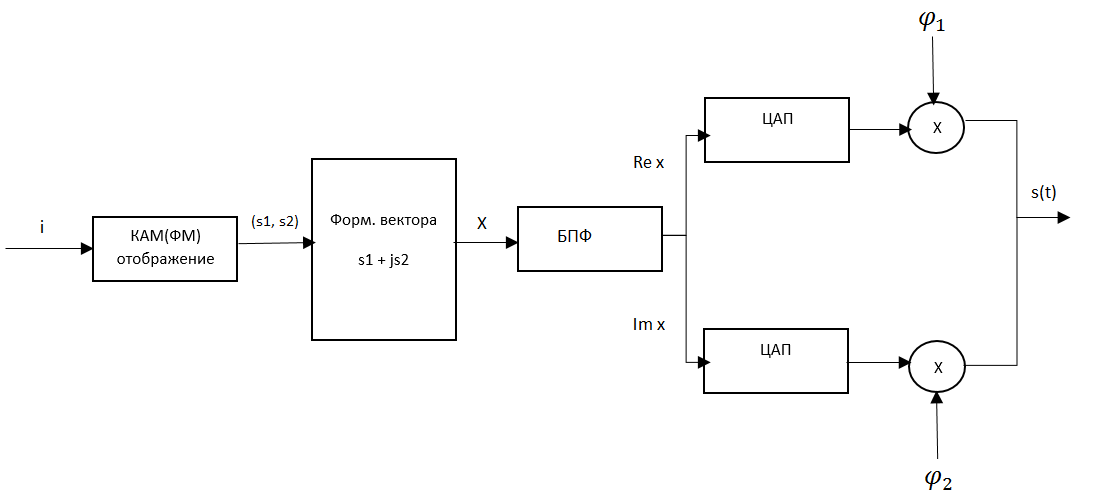
\includegraphics[scale=0.4]{img/Glebov_2.png}
		\caption{Схма формирования сигнала}
		\label{Glebov.image3}
	\end{figure}
	Рассмотрим схему приема сигнала. Принятый сигнал умножается на гармонические функции 
	$\varphi_1=\sqrt{2/T}\cos2\pi f_0t$ и $\varphi_2=-\sqrt{2/T}\sin2\pi f_0t$. 
	Далее аналого-цифровые преобразования формируют векторы $r_1$ и $r_2$. 
	Из векторов $r_1$ и $r_2$ строится комплексный вектор $r_1+jr_2$ и подвергается обратному преобразованию Фурье. 
	По результатам полученного вектора выностится решение о принятом сообщении.
	
	\begin{figure}[h!]
		\centering
		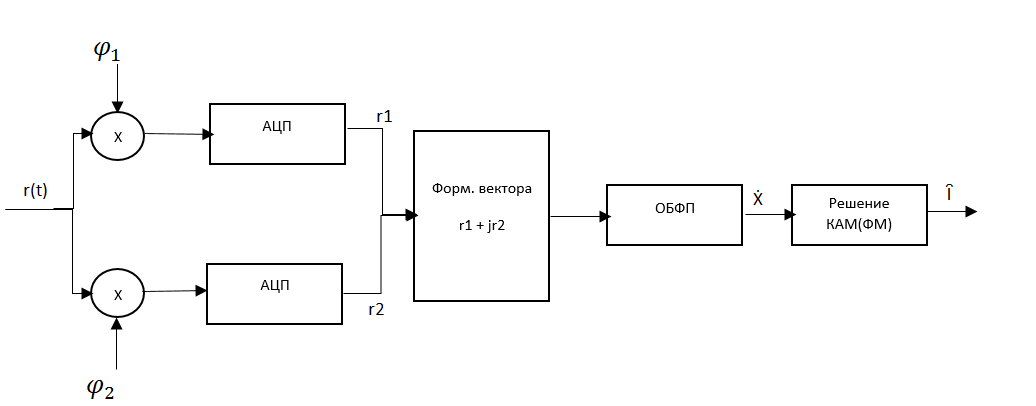
\includegraphics[scale=0.4]{img/Glebov_3.png}
		\caption{Схма приема сигнала}
		\label{Glebov.image4}
	\end{figure}

	На примере двух схем видно, что при использовании комплексного сигнала интегратор не нужен.
	
	
\lstinputlisting[language=Matlab, frame=single,
label=code:Glebov.code1, caption=Листинг программы]
{src/dz2.m}